\chapter{Método gráfico para ajustar uma reta com incerteza}
\label{sec:retagrafico}

\vspace{-0.5cm}

Se medimos ccccccccc duas variáveis, X e Y, cuja relação sabemos que é linear, podemos encontrar uma relação analítica que melhor ajuste nossos dados. No Capítulo juju \ref{histo} da parte Conceitos Básicos na apostila discutimos como isto é feito analiticamente mediante o método de mínimos quadrados, mas aqui estudaremos como faze-lo a partir do gráfico de Y em função de X, o que chamamos de {\bf método gráfico}.

Na figura seguinte podemos observar a distribuição dos dados, círculos abertos, que queremos ajustar. Neste caso, para simplificar, vamos considerar que a incerteza associada a cada medida é do tamanho do ponto.  Para ajustar graficamente os pontos  por uma reta que melhor representa a variação de Y em função de X devemos traçar uma reta de forma tal que os pontos que se situem ``acima" da reta se vejam compensados pelos pontos que se situem ``abaixo'' da mesma, como na linha cheia mostrada na figura~\footnote{Note que o uso de uma régua transparente é conveniente pois permite ter uma visão global de todos os pontos.}. 
\begin{figure}[!h]
\vspace{-0.4cm}
\begin{center}
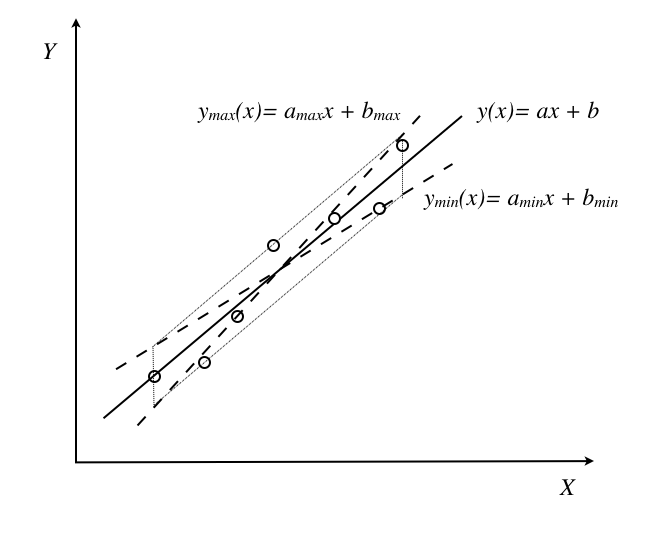
\includegraphics[width=9cm]{fig/GraficoLinGrafico}
\vspace{-0.4cm}
\end{center}
\end{figure}


Desta forma podemos determinar o coeficiente angular ($a$) e linear ($b$) para a equação da reta $y = ax + b$.  Mas mesmo no caso gráfico é preciso dar as incertezas associadas à determinação de $a$ e $b$.  Para isto, vamos traçar duas linhas paralelas à melhor reta ($R$) que ajusta os nossos dados encontrados, uma passando pelo ponto mais afastado ``acima'' da reta $R$ e outra pelo ponto mas afastado ``abaixo'' da reta $R$. %, formando o paralelepípedo pontilhado tal como é mostrado na figura. 
Caso exista um ou outro ponto excepcionalmente afastado da reta média poderá não ser considerado pois a probabilidade de corresponder a uma medida incorreta é grande. Obtendo a interseção destas retas por duas retas paralelas ao eixo-y que contêm o primeiro e último ponto experimental representado temos um ``paralelogramo de incerteza" como é mostrado na figura (paralelogramo pontilhado). A partir deste, desenhamos as duas retas diagonais achando o que chamaremos a reta de máxima $y_{max} = a_{max} x + b_{max}$ e a de mínima $y_{min} = a_{min} x + b_{min}$ (ver figura).

A partir destas três retas, podemos então determinar as incertezas associadas para o coeficiente angular $\delta a$ e linear $\delta b$ como:
\[
\delta a = \frac{a_{max} - a_{min}}{2} 
\]
\[
\delta b = \frac{b_{max} - b_{min}}{2}
\]